% !TeX spellcheck = en_GB
\chapter{Introduction}
\label{sec:introduction}

\section{Motivation}
In this section, we legitimate this work and explain the value and applicability of our proposed solution.

\section{Background}

% TODO: Write introduction: We work with \cite{ietf-mile-xmpp-grid-05}, which is (as the name suggetss) heavily based on XMPP and some XEPs.

\subsection{XMPP (eXtensible Messaging and Presence Protocol)}
The Extensible Messaging and Presence Protocol (in short XMPP) is an open protocol that enables the near-real-time exchange of small data between any network endpoints\cite{rfc6120}. While it was originally designed for Instant Messaging (IM), it can be an is used for a wide range of data exchange applications \cite{ieee-xplore-stream-xml-xmpp}.

% Should we add concrete examples here? Google Talk, Facebook Chat, Collecta Search Engine (http://collecta.com/) and t IEEE Draft ... (sourcE: proffessional xmpp programming)

XMPP is made of small building blocks defined in the core protocol\cite{rfc6120} and numerous extensions called XEPs \cite{xep-0001}. The core comprises of functionality for setup and encryption of communication channels, XML Streams error handling and more. Addition functionality such as service discovery\cite{xep-0030}, Publish-Subscribe\cite{xep-0060} are defined in additional extensions.

Although XMPP supports peer-to-peer communication it is mostly used in a traditional client-server architecture. A client can send data to any addressable (using Jabber IDs, JIDs) entity. The receiver is not present in the same domain (server), the server negotiates a server-to-server stream and forwards the data to it.\cite{rfc6120}

The data exchanged over XMPP is XML which makes structured as well as extensible. XMPP uses XML in the of unidirectional data streams which are basically long-lived TCP-Connections. The client opens a connection to the server, and the server opens one back (i.e. `<stream>`. In both streams, an XML element is opened after the connection is established. During the conversation, an arbitrary amount of Stanzas (specified XML child elements) written in the stream. Before the connection is closed, the root element is closed (i.e. `</stream>') and the two streams form two valid XML documents.\cite{rfc6120}\cite{professional-xmpp}

The core Stanza types are messages (`<message/>`), presence (`<presence/>`) and Info/Query (`<iq/>'). Messages can contain arbitrary data similar to email but optimised for immediate delivery. Presence deals with network availability and the propagation of presence. An Info-Query consists of a request and a response (similar to the GET and POST HTTP methods), which is used for example for feature negotiation and configuration. Because of these coarse semantics, XMPP provides a generalized communication layer. \cite{rfc6120} \cite{ieee-xplore-stream-xml-xmpp}

Figure \fullref{fig:xmpp-overview} illustrates an example setup with two servers and three clients.

\begin{figure}[h]
	\centering
	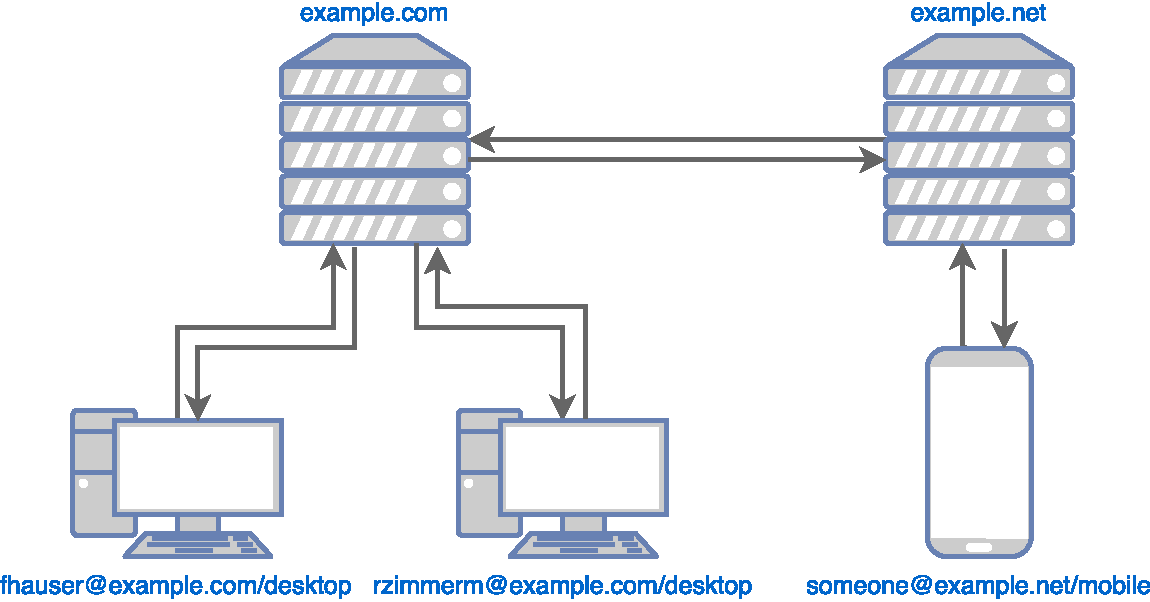
\includegraphics[width=0.8\linewidth]{resources/xmpp_overview.pdf}
	\caption{Two XMPP domains (servers), one with two users and one with one mobile user.}
	\label{fig:xmpp-overview}
\end{figure}

\subsection{Relevant XMPP Extensions}

The XMPP grid draft\cite{ietf-mile-xmpp-grid-05} makes heavy use of multiple XEPs, most notably publish-subscribe. The following XEPs are relevant as well:

\paragraph{XEP-0004: Data Forms} is a flexible protocol that can be used in workflows such as service configuration as well as for application-specific data description and reporting. The protocol provides forms processing, common field types as well as extensibility mechanisms. \cite{xep-0004} 

\paragraph{XEP-0030: Service Discovery} enables applications to discover information about the identity and capabilities of an entity, e.g. is it a server, as well as items associated with an entity, e.g. a list of publish-subscribe nodes. \cite{xep-0030}

\paragraph{XEP-0059: Result Set Management} allows entities to manage the receipt of large result sets, e.g. by paging through the result or limiting the number of results. Result Management is often desired when dealing with large dynamic result sets from service discovery or publish-subscribe and time or other resources are limited. \cite{xep-0059} 

\subsubsection{XEP-0060: Publish-Subscribe}

The Publish-Subscribe Extension, hereafter called PubSub, enables XMPP entities broadcast information via nodes to subscribed entities. \cite{xep-0060}

Nodes, also known as topics and exchanges, are the communication hubs. Entities can create nodes and configure them, e.g. set up subscription timeouts, limit publish and subscription rights. The configuration mechanism is based on data forms (XEP-0004).

The protocol defines a hierarchy of six affiliations of which only two, `owner` and `none`, and are required. The remaining four affiliations are recommended. An owner of a node can manage the subscriptions as well as affiliations of other entities associated with a given node. % TODO (in Sprint 2): Discuss if this is problematic...

% TODO: This might be extended depending on the further contents of this document
\subsection{IETF Internet-Draft: Using XMPP for Security Information Exchange}
TODO \cite{ietf-mile-xmpp-grid-05}
